%Copyright 2014 Jean-Philippe Eisenbarth
%This program is free software: you can 
%redistribute it and/or modify it under the terms of the GNU General Public 
%License as published by the Free Software Foundation, either version 3 of the 
%License, or (at your option) any later version.
%This program is distributed in the hope that it will be useful,but WITHOUT ANY 
%WARRANTY; without even the implied warranty of MERCHANTABILITY or FITNESS FOR A 
%PARTICULAR PURPOSE. See the GNU General Public License for more details.
%You should have received a copy of the GNU General Public License along with 
%this program.  If not, see <http://www.gnu.org/licenses/>.

%Based on the code of Yiannis Lazarides
%http://tex.stackexchange.com/questions/42602/software-requirements-specification-with-latex
%http://tex.stackexchange.com/users/963/yiannis-lazarides
%Also based on the template of Karl E. Wiegers
%http://www.se.rit.edu/~emad/teaching/slides/srs_template_sep14.pdf
%http://karlwiegers.com

%Modified for EECS 393 project in Spring 2017
%Dina Benayad-Cherif, Jason Dong, Mark Lalor, Yousef Mahmoud, Vimig Socrates
\documentclass{scrreprt}

\usepackage[T1]{fontenc}
\usepackage[utf8]{inputenc}

\usepackage{graphicx}

\usepackage{listings}
\usepackage{xcolor}
\usepackage[bookmarks=true]{hyperref}
\usepackage[english]{babel}
\usepackage[utf8]{inputenc}
\usepackage[english]{babel}

\hypersetup{
    bookmarks=false,
    pdftitle={Software Design Document},
    pdfauthor={Dina Benayad-Cherif, Jason Dong, Mark Lalor, Yousef Mahmoud, Vimig Socrates},
    pdfsubject={EECS 393 Software Design Document},
    pdfkeywords={SRS, Software, Design},
    colorlinks=true,        % false: boxed links; true: colored links
    linkcolor=blue,         % color of internal links
    citecolor=black,        % color of links to bibliography
    filecolor=black,        % color of file links
    urlcolor=purple,        % color of external links
    linktoc=page            % only page is linked
}

\addto\captionsenglish{\renewcommand{\contentsname}{Table Of Contents}}
\def\myversion{1.0}
\date{}

\begin{document}

% Title Page
\begin{flushright}
	\rule{16cm}{5pt}\vskip1cm
	\Huge{SOFTWARE DESIGN\\ DOCUMENT}\\
	\vspace{2cm}
	for\\
	\vspace{2cm}
	Class Collaboration Application (CCA)\\
	\vspace{2cm}
	\LARGE{Release \myversion \\}
	\vspace{2cm}
	Prepared by Dina Benayad-Cherif, Jason Dong, Mark Lalor, Yousef Mahmoud, Vimig Socrates\\
	\vfill
	\rule{16cm}{5pt}
\end{flushright}

\tableofcontents

%%%%%%%%%%%%%%%%
% INTRODUCTION %
%%%%%%%%%%%%%%%%

\chapter{Introduction}

\section{Purpose}
This design document describes the overall structure of the Class Collaboration Application (CCA) by outlining significant aspects of the system’s architecture.


\section{Scope}
This application will be used for students at Case Western Reserve University to collaborate and discuss specific courses they are in with other students. Some of the key features of this application are that students will be able to chat with other students in the course, upload class notes or other miscellaneous documents to discuss, and ask questions. Users will also be able to download any documents uploaded for a course that they are enrolled in and can personalize their own account on the CCA. 

\section{Acronyms, Abbreviations and Definitions}
\textit{CCA (Class Collaboration Application)} - Acronym of the name of the application.  \\
\textit{PaaS (Platform as a Service)} - Acronym of a cloud computing platform. \\
\textit{IaaS (Infrastructure as a Service)} - Acronym of a cloud computing infrastructure.\\
\textit{VM (Virtual Machine)} - Acronym of virtual machine. \\
\textit{SSO (Single Sign-On)} - Acronym of a tool for access control across several independent software systems. 

\section{Overview}
This document is an overview of the software architecture of the Class Collaboration Application in high detail. We start by providing all the principal classes that the application is built on as well as their responsibilities to the success of the application. Next, we provide diagrams to show the hierarchy of our classes and the archeitectural design. After, we built an general API of the major class methods used to build the functionality of our application. There are also mockups of our UI design included in our design document. 

\section{Reference Material}
\textit{Book Inventory System System Design Document.} December 8 2010. \\
ZZZ Company. \textit{ZZZ Software Architecture.} October 2 2015. 


%%%%%%%%%%%%%%%%%%%
% SYSTEM OVERVIEW %
%%%%%%%%%%%%%%%%%%%

\chapter{System Overview}

%%%%%%%%%%%%%%%%%%%%%
% PRINCIPAL CLASSES %
%%%%%%%%%%%%%%%%%%%%%

\chapter{Principal Classes}
	
\section{Student}
The student contains all user information including, student ID, the name of the student, the courses they are enrolled in, their username and the last time they logged in. A new student is created by checking whether a specific user has previously logged into the Class Collaboration Application.
\subsection{Responsibilities}
\begin{itemize}
	\item Monitoring the current session of the user.
	\item Querying any user updates to the database. 
	\item Displays all the courses the student is enrolled in. 
	\item Recording when the user has gone idle. 
	\item Uploads and removes documents.
	\item Can create CourseItems for a specific course.
	\item Can join or create courses.
\end{itemize}

\section{Course}
A Course is able to aggregate all of the information and student created objects that are associated with a particular course. Created objects include all of the CourseItem objects associated with the Course and a single Chat object to be used as the general chat for the Course.
\subsection{Responsibilities}
\begin{itemize}
	\item Presenting to the user all CourseItem objects that have been added to the course from all Students 
	\item Presenting the Chat object for the course to allow communication between the Student and all other Students with the chat object
	\item Querying any updates to the Course objects and updating the CourseItem and Chat objects
\end{itemize}

\section{CourseItem}
A course item is an assignment, exam, URL, or other document relevant to the course. The CourseItem is a created object that is created by a user in the Student class and will be shared through a Course’s chat object and always accessible on the sidebar. The user who created the CourseItem object will be able to later modify or delete the object.
\subsection{Responsibilities}
\begin{itemize}
	\item Display to the user the name and description of the courseItem
	\item Allow the creator of the courseItem to modify or delete the courseItem
	\item Query any updates to the courseItem and update the courseItem accordingly
	\item Provide a download option so that a Student can download the contents of a course item
\end{itemize}

\section{Chat}
A chat is created for each Course and for each CourseItem. Chats are not created by or associated with users in any way, they are only automatically created/exist alongside existing Courses and CourseItems.
\subsection{Responsibilities}
\begin{itemize}
	\item Tracking and recording to the database new messages in the chat. Messages are written to the database immediately (are not written to a buffer/flushed).
	\item Notifying the client of changes when the client checks (asks) whether any changes (new messages) have occurred.
	\item Providing specific messages upon request.
	\item Caching messages as they are accessed to reduce read operations on the database.
\end{itemize}

%%%%%%%%%%%%%%%%%%%%%%%
% SYSTEM ARCHITECTURE %
%%%%%%%%%%%%%%%%%%%%%%%

\chapter{System Architecture}

\section{Architectural Design}

\begin{figure}[ht]
  \centering
  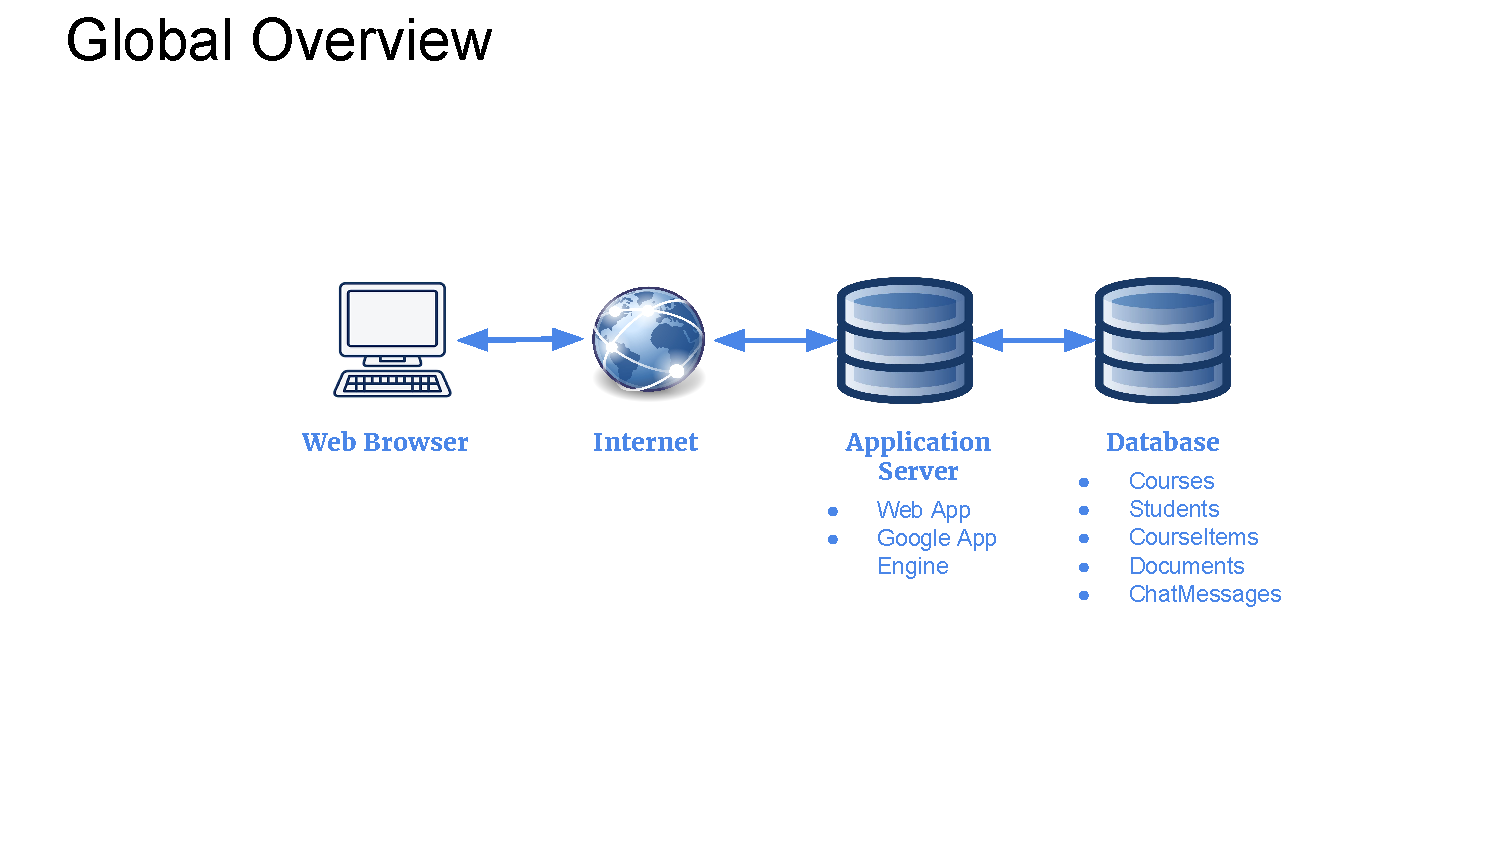
\includegraphics[page=1,width=0.9\textwidth]{diagrams/SDD_Diagrams.pdf}
  \label{fig:SDD_1}
\end{figure}

\begin{figure}[ht]
  \centering
  \includegraphics[page=2,width=0.9\textwidth]{diagrams/SDD_Diagrams.pdf}
  \label{fig:SDD_1}
\end{figure}

\begin{figure}[ht]
  \centering
  \includegraphics[page=3,width=0.9\textwidth]{diagrams/SDD_Diagrams.pdf}
  \label{fig:SDD_1}
\end{figure}

\section{Decomposition Description}

\section{Design Rationale}
\hspace{10mm}We decided to use Google App Engine because it is a reliable platform to scale and build web applications. Many web applications are maintained either through IaaS or PaaS. We decided not to use Iaas because, although we can have root access to a VM, we would have to be responsible for managing the resources on the machine including, memory and CPU usage. Since Google App Engine is a PaaS, it manages all of our computational resources for us, so our only responsibility is maintaining the application while Google App Engine would take care of the infrastructure, security and scalability of the Class Collaboration Application. 

\hspace{10mm}For each user, we decided to integrate SSO into our application. Using SSO as a way for users to sign into the application through their Case credentials boosts our security capabilities as well as mitigates the risk of 3rd party applications accessing sensitive information about the user. This also improves user experience where the user does not have to create and keep track of another username and password. 


%%%%%%%%%%%%%%%%%%%%
% CLASS INTERFACES %
%%%%%%%%%%%%%%%%%%%%

\chapter{Class Interfaces}

\section{Class Student}
An instance of Student represents a user who can create CourseItems and 		Courses. A student is also able to upload Documents attached to a CourseItem.

\subsection{Public Constructor Student}
\textit{Student(String name, String id, Time lastLogin)} \\
Creates a student object containing the name and Case ID.

\subsection{Public Method GetStudentID}
\textit{String GetStudentID()} \\
Returns the Case ID of the user.

\subsection{Public Method GetDurationOfSession}
\textit{Time GetDurationOfSession()} \\
Returns the length of the current login session of the user.

\subsection{Public Method IsSessionExpired}
\textit{Boolean IsSessionExpired()} \\
Returns whether the the current login session is expired.

\subsection{Public Method CreateCourseItem}
\textit{Boolean CreateCourseItem(dict options, Course course)} \\
Creates an instance of a CourseItem and returns whether it was 		successfully made.

\subsection{Public Static Method CreateCourse}
\textit{Boolean CreateCourse(String courseID, String CourseName)} \\
Creates an instance of a Course and returns whether it was			 successfully made.

\subsection{Public Method GetEnrolledCourses}
\textit{List<Course> GetEnrolledCourses()} \\
Returns the list of courses a student is currently enrolled in on the application.

\subsection{Public Method JoinCourse}
\textit{Boolean JoinCourse(Course course)} \\
Returns whether a student successfully joined to a preexisting course.

\section{Class Course}

\subsection{Public Constructor Course}
\textit{Course(String courseID} \\
Creates a Course object from the supplied courseID. Populates private fields with items from the database queried using courseID.

\subsection{Public Method GetStudents}
\textit{List<Student> GetStudents()} \\
Queries the students table of the database to see which students have added this course to their list of courses.

\subsection{Public Method GetCourseItems()}
\textit{List<CourseItem> GetCourseItems()} \\
Queries the database to return a list of all CourseItems associated with the course.

\subsection{Public Method GetChat}
\textit{Chat GetChat()} \\
Returns the instance of the Chat class associated with the Course.

\section{Class CourseItem}
An object created by a student that can contain a document relevant to the course. This object is associated with a Course object.

\subsection{Public Method RemoveCourseItem}
\textit{Boolean RemoveCourseItem()} \\
Removes the CourseItem from the database, so that it is no longer available to Students.

\subsection{Public Method ModifyCourseItem}
\textit{Boolean ModifyCourseItem(Document document)} \\
Adds the document to the already existing CourseItem.

\section{Class Document}

\subsection{Public Constructor Document}
\textit{Course(Integer documentID} \\
Creates a Document object associated with the specified document ID. This ID is used to query the database to locate the actual file associated with it.

\subsection{Public Method Download}
\textit{Void Download()} \\
Outputs the binary data for the document along with the proper HTTP header (application/octet-stream) to tell the browser to download the file instead of display it.

\subsection{Public Method GetCourseItemID}
\textit{String GetCourseItemID()} \\
Returns the unique id associated with the course item.

\section{Class Chat}
Represents the chat for a course. The Chat object will hold all ChatMessage objects for a course.

\subsection{Public Constructor Chat}
\textit{Chat(String courseID)} \\
Creates a Chat object from the supplied courseID. Populates private fields with items from the database queried using courseID. Since there is one chat per course it is ok to use the courseID as a lookup for Courses as well as Chats.

\subsection{Public Method GetChatVersion}
\textit{Integer GetChatVersion()} \\
Returns what number message the chat has currently advanced to. This is cached whenever possible and queried often by the user to know when to request updates.

\subsection{Public Method GetChatMessages}
\textit{List<ChatMessage> GetChatMessages(Integer number = 50)} \\
Returns that last \textit{number} chat messages associated with this chat (default 50).

\subsection{Public Method SendMessage}
\textit{Void SendMessage(String content, Student author)} \\
Creates a ChatMessage object with a string content and sends it to the chat.

\subsection{Public Method SendDocument}
\textit{Void SendDocument(Document doc, Student author)} \\
Creates a ChatMessage object with a document attached and sends it to the chat.

\section{Class ChatMessage}
Represents a single message sent in a Chat. This message can be text or a document.

\subsection{Public Constructor ChatMessage}
\textit{Chat(String courseID)} \\
Creates a ChatMessage object associated with the courseID.

\subsection{Public Enum MessageType}
\textit{} \\
Indicates the chat message type. Currently can be:
\begin{itemize}
	\item Text
	\item Document
	\item Image
\end{itemize}

\subsection{Public Method GetType}
\textit{MessageType GetType()} \\
Returns the type of the message.

\subsection{Public Method GetContent}
\textit{Void GetContent()} \\
Returns the content associated with the ChatMessage.

\subsection{Private Method GetText()}
\textit{String GetText()} \\
Returns the text associated with this ChatMessage

\subsection{Private Method GetURL()}
\textit{String GetURL()} \\
Returns the URL associated with this ChatMessage.

\subsection{Public Method GetStudent}
\textit{Student GetStudent()} \\
Returns the Student who created the ChatMessage object.

\subsection{Public Method GetTime}
\textit{Time GetTime()} \\
Returns the time the ChatMessage object was sent.

\subsection{Public Method Delete()}
\textit{Void Delete()} \\
Removes the ChatMessage object from the database. This object will no longer be shown in the Chat object class.

%%%%%%%%%%%%%%%%%%%%%%%%%%
% HUMAN INTERFACE DESIGN %
%%%%%%%%%%%%%%%%%%%%%%%%%%

\chapter{Human Interface Design}

\section{Mockup of User Interface}

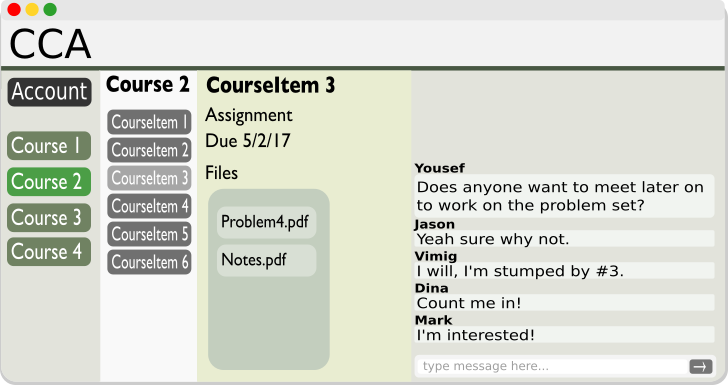
\includegraphics[width=1.0\textwidth]{diagrams/UI_Mockup.png}


\end{document}
